\documentclass{beamer}

\usepackage[utf8]{inputenc}
\usecolortheme{beaver}
\usepackage{caption}
\usepackage{subcaption}
\usepackage{mathtools}
\usepackage{todonotes}
\usepackage{amsmath}
\usepackage{bm}
\usepackage{listings}
\usepackage{ragged2e}
\usepackage{titlecaps}
\usepackage{fancyvrb}

\def\ci{\perp\!\!\!\!\!\perp}

\newtheorem{proposition}{Proposition}
\Addlcwords{for a is but and with of in as the etc on to if}

\setbeamertemplate{section in toc}{\inserttocsectionnumber.~\inserttocsection}
\usetheme{Boadilla}
\makeatletter
\setbeamertemplate{footline}{%
    \leavevmode%
    \hbox{%
        \begin{beamercolorbox}[wd=.3\paperwidth,ht=2.25ex,dp=1ex,center]{author in head/foot}%
            \usebeamerfont{author in head/foot}\insertshortauthor\expandafter\beamer@ifempty\expandafter{\beamer@shortinstitute}{}{~~(\insertshortinstitute)}
        \end{beamercolorbox}%
        \begin{beamercolorbox}[wd=.55\paperwidth,ht=2.25ex,dp=1ex,center]{title in head/foot}%
            \usebeamerfont{title in head/foot}\insertshorttitle
        \end{beamercolorbox}%
        \begin{beamercolorbox}[wd=.15\paperwidth,ht=2.25ex,dp=1ex,right]{date in head/foot}%
            \usebeamerfont{date in head/foot}\insertshortdate{}\hspace*{2em}
            \insertframenumber{} / \inserttotalframenumber\hspace*{2ex} 
        \end{beamercolorbox}}%
        \vskip0pt%
    }
\makeatother


\begin{document}

\title[]{Causal Reasoning and Large Language Models: Opening a New Frontier for Causality}
\author {}
\date{}
\maketitle

\begin{frame}
	\frametitle{Abstract}
	\begin{enumerate}
		\item LLM-Based methods establish new state-of-the-art accuracy on multiple causal benchmarks.
		\item Outperforms existing algorithms on: 1) Pairwise causal discovery, 2) Counterfactual Reasoning, 3) Actual causality
		\item But exhibits unpredictable failure modes.
		\item Envisons LLMs to be used alongside existing causal
			methods, as a proxy for human domain knowledge.
		\item Also see existing causal methods as promising tools for LLMs to
			formalize, validate, and communicate their reasoning.
		\item Paper doesn't imply that complex causal reasoning has
			emerged in LLMs. But it has captured common sense and
			domain knowledge from natural language.
	\end{enumerate}
\end{frame}

\begin{frame}
	\frametitle{Introduction}
	\begin{enumerate}
		\item Paper explores what kind of causal reasoning might LLMs
			be performing, if they are, what are the purposes for
			which they might be employed, if they can be?
		\item Proposes a framework for future research at the intersection of
			LLMs and causality.
		\item Begins with a recognition of different kinds of causal knowledge 
			and reasoning implicated in this debate, including prior knowledge
			of general and domain-specific knowledge.
		\item Claims that LLMs bring significant new capabilities which
			are complementary to existing causal methods.
	\end{enumerate}
\end{frame}

\begin{frame}
	\frametitle{Summary of Results}
	\begin{enumerate}
		\item Causal Discovery
			\begin{itemize}
				\item Pairwise causal discovery: Outperforms 97 \% vs 83 \% on Tubingen benchmark.
				\item Full graph: Competitive to recent methods
			\end{itemize}
		\item Actual Causality: Considers individual events and aims to find
			what caused them.
			\begin{itemize}
				\item Involves simulation of different
					counterfactual scenarios.
				\item Perfoms better for most benchmarks except the ones
					that require an understanding of human factors.
			\end{itemize}
	\end{enumerate}
	Makes surprisingly few mistakes given that it doesn't even use actual data but just the metadata.
\end{frame}

\begin{frame}
	\frametitle{Implications for causality research}
	\begin{enumerate}
		\item Conventional causal discovery and effect inference rely strongly on prior domaning knowledge of potential causal mechanism. 
		\item Current best practice relies on human domain experts to provide this knowledge.
		\item Capturing domain knowledg in a formal representation suitable for analysis remains a challenge.
		\item LLMs allow access to an array of memorized or inferred causal mechanisms, capturing general and domain-specific knowledge and may augment human experts by aiding in bootstrapping, critiquing, etc.
		\item LLMs do have unexpected failure modes. In all the tasks studies, LLMs achive high average accuracies but also make simple, unpredictable mistakes on certain inputs.
		\item Accuracy depends on the prompt used.
		\item Further research is needed to understand when LLM outputs can be trusted and increase their robustness.
	\end{enumerate}
\end{frame}

\begin{frame}
	\frametitle{Background: Types of Causality}
	\begin{enumerate}
		\item Covariance-based Causality: Uses statistical
			approaches to discover and estimate the strengths of
			causal relationships from data. E.g. Drug efficacy, effects 
			of novel economic policies
		\item Logic-Based Causality: Fields like law, forensics, fault diagnosis
			often emphasize logic-based causality, which uses logical
			reasoning and domain knowledge to reason about the causal 
			relationships in systems.
		\item Type and Actual Causality: Type causality encompasses inference
			on causal relationships between variables, such as in causal 
			discovery and causal effect estimatio. In contrast, actual 
			causality refers to inference of the degreee to which specific
			events cause other events. Questions like "Was Fred's smoking 
			habit responisble for his lung cancer?"
	\end{enumerate}
\end{frame}

\begin{frame}
	\frametitle{Background: Different Causal Tasks and their connections to kinds of causality}
	Some of the causal inference tasks.
	\begin{enumerate}
		\item Causal Discovery: The task of recovering the underlying causal
			mechanism that govern a system. Primarly covariance-based in the
			context of type causality.
		\item Effect Inference: Task of characterizing the strength and shape of 
			a known or hypothesized causal relationship. \todo[inline]{Maybe add more to this}
		\item Attribution: Task of determining the cause of a change. Depending on the applicatio domain, usually involves both covariance based and logic based approaches.
		\item Judgement tasks: Extend attribution tasks to question of reward or
			blame assignment for outcomes.
	\end{enumerate}
\end{frame}

\begin{frame}
	\frametitle{LLMs and Causality}
	\begin{enumerate}
		\item First, the paper investigates the graph discovery capabilities of
			LLMs over a broad set of complex real-world tasks.
		\item Second, the paper probes the ability of LLMs to do counterfactual
			reasoning and infer necessary or sufficient cause based on
			natural language description of the world.
	\end{enumerate}
\end{frame}

\begin{frame}
	\frametitle{Probing LLM behaviors}
	\begin{enumerate}
		\item Since LLMs are text based, the main way to understand its causal
			capibiilities is to probe it with different inputs and observe
			how the output changes.
		\item This paradigm has the classic limitation of construct
			validity for the measurements. That is we may be
			tempted to ascribe a particular causal capability to an
			LLM if it answers well on a set of questions related to
			the capability.
		\item Tests the capabiility on standard benchmark datasets and also
			does memoization tests on the LLM to test the extent to which
			the LLM has memoized the benchmark. Construct novel datasets, and
			do perturbations to test whether the LLM is memoizing.
	\end{enumerate}
\end{frame}

\begin{frame}
	\frametitle{Benchmark Tests and Question-Answer Evaluation}
	\begin{enumerate}
		\item Give a prompt to the LLM and the completion of the prompt is 
			the answer.
		\item For each evaluation, we ask a series of questions or causal 
			challenges and score the correctness of the resulting answer.
	\end{enumerate}
\end{frame}

\begin{frame}
	\frametitle{Memorization Test}
	\begin{enumerate}
		\item The primary treat to the validity of benchmark or question-answer
			style assessments is that the LLM may have directly 
			memorized the benchmark answers.
		\item To test whether the LLM has memorized a particular dataset
			or benchmark, we give the LLM a partial row of data from
			the dataset and ask it to complete the remaining.
		\item For question-answer taks half of the question and ask it to 
			complete the rest.
		\item To encourage the LLM to succeed, we prepend details about the
			dataset, such as its name, URL, and description, and also
			provide few-shot examples.
	\end{enumerate}
\end{frame}

\begin{frame}
	\frametitle{Redaction Test}
	\begin{enumerate}
		\item To better understand what aspets of the prompt or
			question an LLM is attending to, we use redaction and
			perturbation tests.
		\item First, we redact words in the prompt, one by one, and see how 
			the answers change each time. Changes in the answer indicate
			the LLM is attending to the redacted word.
	\end{enumerate}
\end{frame}

\begin{frame}
	\frametitle{LLMs and Causal Discovery}
	\begin{enumerate}
		\item Having the correct causal graph that encodes causal assumptions
			is critical for ensuring the correctness of any downstream
			analysis.
		\item Generally it is not possible to learn the correct graph for
			a given dataset, given only observational dataset.
		\item A set of graph structures known as Markov Equivalence
			class are equally likely given the same observational
			data distribution.
		\item Two main approaches to overcome this issue:
			\begin{itemize}
				\item Restrict data-generating process to a specific
					functional form under which identification
					of a single graph is possible.
				\item Use deep learning to model the covariances of
					all variables jointly and hope that it improves
					the quality of learned graphs.
			\end{itemize}
		\item LLMs offer a fresh perspective on the causal discovery problem
			by focusing on the metadata associated with variables in a 
			dataset, rather than their data values.
		\item Usually domain experts can use such meta data along with the 
			context to construct causal structures. LLM does the same 
			thing.
	\end{enumerate}
\end{frame}

\begin{frame}
	\frametitle{Pariwise causal discovery: T\"{u}bingen cause-effect pairs dataset}
	\begin{itemize}
		\item 108 different cause-effect pairs selected from 37 datasets from
			various domains, including meteorology, biology, medicine, 
			engineering, and economics.
		\item Markov equivalence class contains both $ A \rightarrow B $ and 
			$ B \rightarrow A $.
		\item Use names of the variables to construct the LLM query.
		\item Start with simple prompts that asks ``Does changing $ A $ cause a change in $ B $?''. 
		\item For any given pair $ (A , B) $, the query is asked in both
			directions and then take the mean accuracy.
		\item If both answers are wrong, accuracy is $0$. If one is correct, 
			it chooses at random.
		\item Two different kinds of prompts: 1) Prepend the prompt with the 
			message, ``You are a helpful assistant for causal reasoning''. 2)
			Asking the LLM to output the more likeliy causal direction
			between $ A \rightarrow B $ and $ B \rightarrow A $ while
			explaining the reasoning in a ``step-by-step'' manner.
	\end{itemize}
\end{frame}

\begin{frame}
	\frametitle{Understanding the LLM output}
	\begin{itemize}
		\item Done on the single prompt only.
		\item Can sometimes make errors but surprisingly made only
			12 errors in the dataset of 108 pairs.
		\item In some cases, the LLMs output doesn't match the ground truth
			but it revels possible ambiguity in the variable names that 
			can be fixed by adding more context to the question.
		\item \todo[inline]{Add the ozone example}
		\item \todo[inline]{Add the HSBC example where the caus-effect
			relationship is not absolute}
	\end{itemize}
\end{frame}

\begin{frame}
	\frametitle{Neuropathic pain dataset}
	\begin{itemize}
		\item In the previous dataset the variable names are very common and
			can be understood by most of the people.
		\item This dataset is more domain specific compared to the Tubingen.
		\item The dataset contains relationship between different nerves and 
			the associated symptoms that the patients express.
		\item Similar evaluation as the previous datasets.
		\item 475 edges
		\item The performance of all the text genration engines degrades but
			chat based models, trained on human feedback, are able to 
			distinguish causal direction accurately.
		\item \todo[inline]{Add the results table here}
		\item The choice of prompt has a huge impact on the performance of the
			model.
		\item gpt-4 gets 96\% accuracy yielding more than 457 correct responses
			out of 475.
	\end{itemize}
\end{frame}

\begin{frame}
	\frametitle{Understanding the output}
	\begin{itemize}
		\item It correctly understands the medical terms in almost all cases.
		\item However provides erroneous output in unpredictable ways.
		\item LLMs may not be capable of consistent and coherent reasoning, even
			as they output correct answers for a majority of the causal 
			questions.
		\item \todo[inline]{Show table 5}
	\end{itemize}
\end{frame}

\begin{frame}
	\frametitle{Full graph discovery: How to do a full graph discovery}
	\begin{itemize}
		\item With the pairwise case, we knew that the edge exists and we 
			only needed to determine the direction.
		\item In this case, three different scenarios are possible: 1) Edge in
			either direction 2) No edge exists.
		\item Secondly, we need to distinguish between direct and
			indirect effects. For example, if the True relationship is
			$ A \rightarrow B \rightarrow C $, then in a pairwise task
			it is okay to output both $ A \rightarrow B $ and $ A \rightarrow
			C $ in a pairwise task.
		\item Edges can also depend on which variables are included in the 
			model. For example if $ B $ is not included in the above 
			example $ A \rightarrow C $ is a valid edge.
		\item Because of these reasons it is unclear how exactly to extend the 
			pairwise task to a full graph case.
		\item For smaller graphs with 3-4 variables, papers available on how 
			to do it.
	\end{itemize}
\end{frame}

\begin{frame}
	\frametitle{Neuropathic pain dataset}
	\begin{itemize}
		\item The dataset has 221 variables with a total possible variable 
			pairs of $ C(221, 2) = 24310 $.
		\item Utilize a smaller 100 pair dataset. 50 pairs form edges in the
			graph and 50 pairs do not form an edge.
		\item Many of the names are in Swedish, so uses an LLM to translate 
			the names to english.
		\item In a previous paper with the prompt, ``A causes B. R and L refer
			to the right and left sides of the body respectively. Answer
			True or False.'', they got results worse than random guessing.
		\item With a similar single prompt as in the pairwise case with an 
			additional option: ``C: No causal relationship exists'', results
			in much better performance.
		\item \todo[inline]{Add table 6}
	\end{itemize}
\end{frame}

\begin{frame}
	\frametitle{Arctic Sea ice dataset}
	\begin{itemize}
		\item Dataset on drivers of arctic sea ice thickness/coverage. 
			What causes the arctic ice coverage to increase or decrease.
		\item An expert model used as the ground truth for the dataset with 
			12 variables and 48 edges.
		\item The graph contains some double-sided edges.
		\item Since the number of variables are low, we can do a full 
			graph discovery.
		\item \todo[inline]{Insert table 7}
		\item For LLM based discovry, the same single prompt is used.
	\end{itemize}
\end{frame}

\begin{frame}
	\frametitle{Probing the LLM: Memorization Test}
	To test whether the LLM has memorized the benchmark datasets.
	\begin{itemize}
		\item Provide the LLM with the first 3 columns of the dataset:
			row ID and 2 variable names. And ask the model to
			complete the remaining 2 columns of the row.
		\item GPT-3.5 is able to correctly recall 58\% of the remaining
			cells in the dataset, and recall 19\% of the rows
			without error. GPT-4 with 61\% of the remaining cells
			and 25\% of rows without error.
		\item However the gap between percentage of inputs memorized and LLMs
			accuracy is still significant.
		\item Expect LLMs abilities to be dependent partially on memorizaton
			but partially on ability to process and transform seen
			causal relationship in multiple contexts.
	\end{itemize}
\end{frame}

\begin{frame}
	\frametitle{Probing the LLM: Redaction Test}
	\begin{itemize}
		\item To characterize whether LLM is attending to the correct words.
		\item \todo[inline]{Include Figure 4}
		\item If the LLM is correctly reading the question, we would expect
			that it would pay a lot of attention to the key instructions and
			to the options iteself.
	\end{itemize}
\end{frame}

\begin{frame}
	\frametitle{Pairwise Causal Discovery: T\"{u}bingen cause-effect pairs dataset}
	\begin{itemize}
		\item Given a dataset on $ 2 $ variables, determine the direction of causality.
			$$ (X, Y) \implies X \rightarrow Y \;\; \textit{or} \; \; X \leftarrow Y $$
		\item Not possible to determine the direction without making some assumptions using statistical methods.
		\item 108 cause-effect pairs selected from 37 datasets from
			various domains.
	\end{itemize}
	\begin{figure}
		\centering
		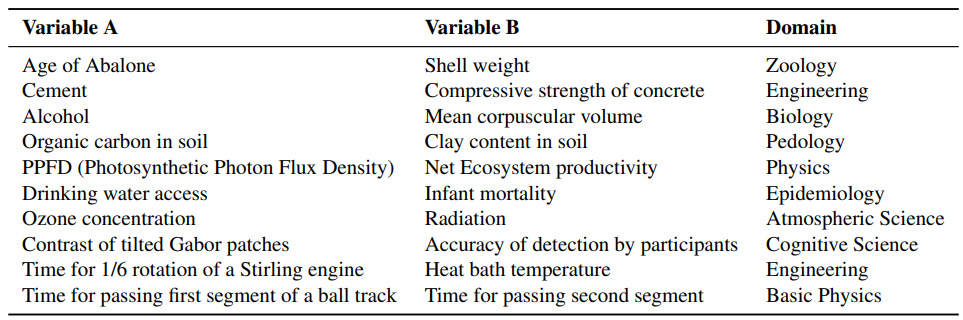
\includegraphics[scale=0.5]{imgs/table1.png}
	\end{figure}
\end{frame}

\begin{frame}
	\frametitle{Pairwise Causal Discovery: T\"{u}bingen cause-effect pairs dataset}
	\begin{itemize}
		\item With the LLM, for any given pair $ (A, B) $ a query is asked: ``Does changing A cause a change in B?''
		\item Ask the query in both the directions and take the mean accuracy.
		\item Two other prompts are used:
			\begin{enumerate}
				\item Prepend the previous prompt with: ``You are a helpful assistant for causal reasoning''.
				\item Asking the LLM to output the more likely causal direction between $ A \rightarrow B $ and $ B \rightarrow A $ while
					explaining the reasoning in a ``step-by-step'' manner.
			\end{enumerate}
	\end{itemize}
\end{frame}

\begin{frame}
	\frametitle{Pairwise Causal Discovery: T\"{u}bingen cause-effect pairs dataset}
	\begin{figure}
		\centering
		\begin{subfigure}{0.5 \textwidth}
			\centering
			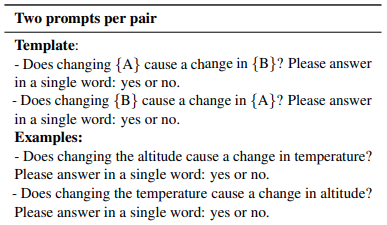
\includegraphics[scale=0.4]{imgs/example1.png}
		\end{subfigure}%
		\begin{subfigure}{0.5 \textwidth}
			\centering
			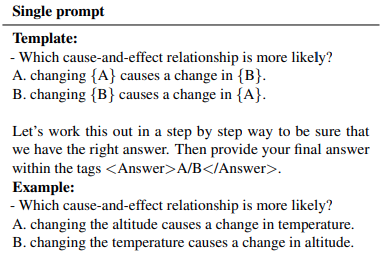
\includegraphics[scale=0.4]{imgs/example2.png}
		\end{subfigure}
	\end{figure}
\end{frame}

\begin{frame}
	\frametitle{Pairwise Causal Discovery: T\"{u}bingen cause-effect pairs dataset}
	\begin{columns}
		\begin{column}{0.5 \textwidth}
			\begin{itemize}
				\item Only 12 errors in 108 pairs with gpt-4.
				\item In some cases, output doesn't match ground truth but reveals possible ambiguity in the variable names.
				\item Providing context in such cases can result in getting the correct answer.
			\end{itemize}
		\end{column}
		\begin{column}{0.5 \textwidth}
			\begin{figure}
				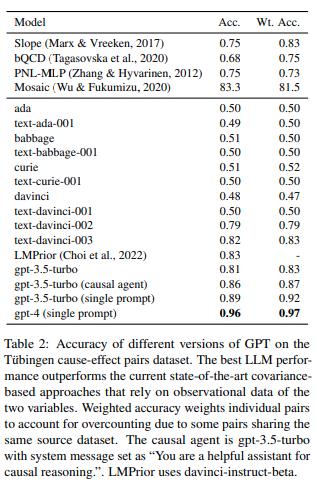
\includegraphics[scale=0.4]{imgs/table2.png}
			\end{figure}
		\end{column}
	\end{columns}
\end{frame}

\begin{frame}
	\frametitle{Pairwise Causal Discovery: Neuropathic Pain Dataset}
	\begin{itemize}
		\item The variable names are more domain specific.
		\item Dataset contains relationship between different nerves and the associated symptoms that patients express.
	\end{itemize}
	\begin{figure}
		\centering
		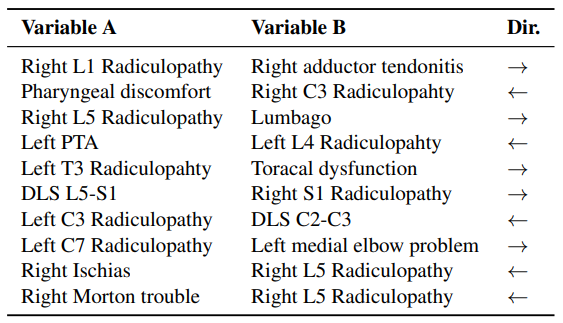
\includegraphics[scale=0.5]{imgs/table3.png}
	\end{figure}
\end{frame}

\begin{frame}
	\frametitle{Pairwise Causal Discovery: Neuropathic Pain Dataset}
	\begin{columns}
		\begin{column}{0.5 \textwidth}
			\begin{itemize}
				\item Performance of text generation engines degrage but chat based models are able to perform better.
				\item gpt-4 gets 457 correct responses out of 475.
			\end{itemize}
		\end{column}
		\begin{column}{0.5 \textwidth}
			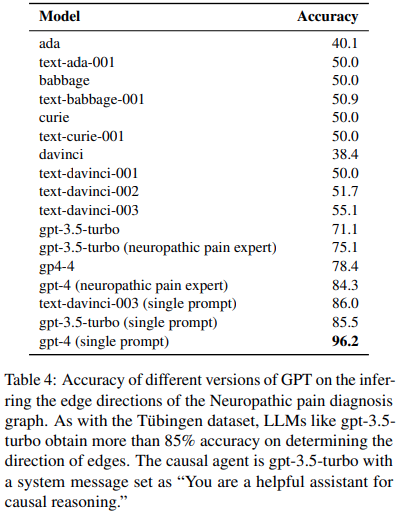
\includegraphics[scale=0.4]{imgs/table4.png}
		\end{column}
	\end{columns}
\end{frame}

\begin{frame}
	\frametitle{Full Graph Discovery}
	\begin{itemize}
		\item Given a dataset, find a DAG representing the causal relationship between the variables.
		\item Three possible scenario between any two variables 1) $ X \rightarrow Y $ 2) $ X \leftarrow Y $ 3) No edge.
		\item Need to also distinguish between direct and indirect effects.
		\item If true relationship is $ A \rightarrow B \rightarrow C $, for pairwise task correct to output $ A \rightarrow B $
			and $ A \rightarrow C $, but not for full graph discovery.
		\item Unclear how to extend pairwise task to a full graph case.
		\item For smaller graphs with 3-4 variables, can iterate over all possible pairs of variables.
	\end{itemize}
\end{frame}

\begin{frame}
	\frametitle{Full Graph: Neuropathic Pain Dataset}
	\begin{itemize}
		\item The dataset has 221 variables, so considering all possible variable pairs is not possible.
		\item Utilize a smaller 100 pair dataset. 50 pairs form edges in the graph and 50 pairs do not form an edge.
		\item Many names are in Swedish, uses an LLM to translate to english as a preprocessing step.
		\item For the prompt an additional option is added as: ``C: No causal relationship exists''.
	\end{itemize}
	\begin{figure}
		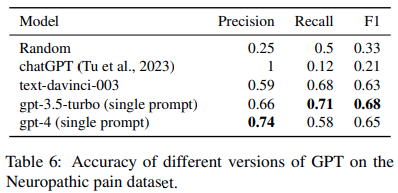
\includegraphics[scale=0.4]{imgs/table6.png}
	\end{figure}
\end{frame}

\begin{frame}
	\frametitle{Full Graph: Arctic Sea Ice Dataset}
	\begin{itemize}
		\item Dataset on driver of arctic sea ice thickness/coverage.
		\item Total of 12 variables and 48 edges with some double-sided edges.
		\item Only ``single prompt'' used for LLMs.
	\end{itemize}
	\begin{figure}
		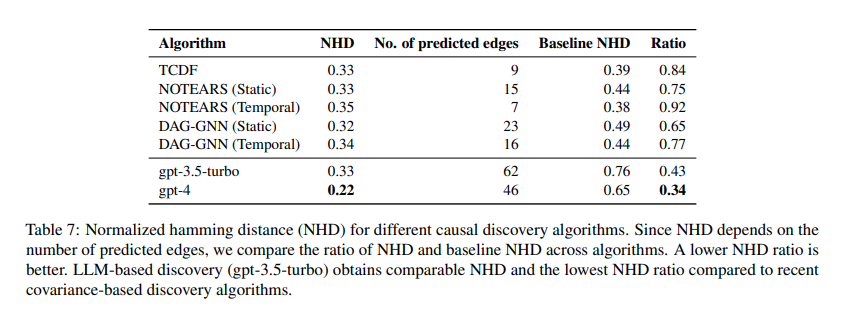
\includegraphics[scale=0.4]{imgs/table7.png}
	\end{figure}
\end{frame}
\end{document}































